\begin{figure}[h]
  \centering
  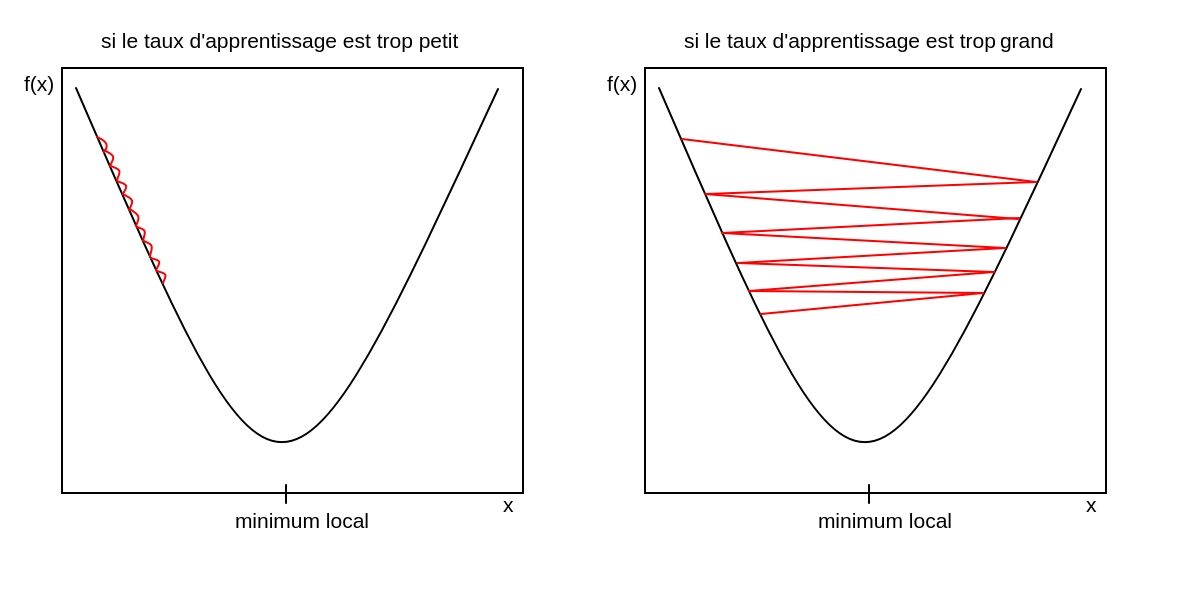
\includegraphics[width=.95\textwidth]{./Chapitre2/figures/tauxApprentissage.png}
  \caption{Exemple de la descente de gradient dans le cas d'un taux d'apprentissage soit trop petit, soit trop grand. L'apprentissage est composé de dix mises à jour des poids.}
  \label{fig:tauxApprentissage}
\end{figure}
